% Beamer slides for Hybrid DPO experiment
\documentclass{beamer}
\usetheme{Madrid}
\usecolortheme{seahorse}
\usepackage{graphicx}
\usepackage{booktabs}
\usepackage{hyperref}
\usepackage{amsmath}
\usepackage{cleveref}
\usepackage{tikz}
\usetikzlibrary{positioning,arrows.meta,shapes.geometric}
\title[Hybrid DPO: Forward+Backward]{Hybrid DPO for Reasoning: Forward + Backward Preference Signal}
\author{Murtaza Nikzad}
\institute{CS Research}
\date{\today}

\begin{document}

\begin{frame}
  \titlepage
\end{frame}
\begin{frame}{Architecture — Encoder}
  \centering
  \vspace{-6mm}
  \resizebox{0.9\textwidth}{!}{%
  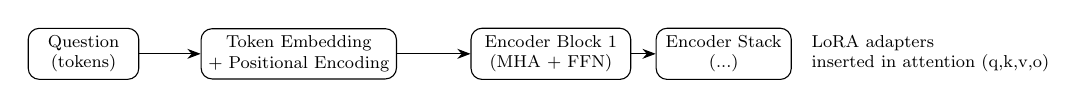
\begin{tikzpicture}[>=Stealth, node distance=4mm, scale=0.78, transform shape, every node/.style={font=\footnotesize}]
    % compact encoder-only diagram
    \node[draw, rounded corners, align=center, minimum width=18mm, minimum height=6mm] (input) {Question\\(tokens)};
    \node[draw, rounded corners, align=center, minimum width=22mm, minimum height=6mm, right=10mm of input] (embed) {Token Embedding\\+ Positional Encoding};

    \node[draw, rounded corners, align=center, minimum width=26mm, minimum height=6mm, right=12mm of embed] (enc1) {Encoder Block 1\\(MHA + FFN)};
    \node[draw, rounded corners, align=center, minimum width=22mm, minimum height=6mm, right=of enc1] (enc2) {Encoder Stack\\(...)};

    \node[font=\footnotesize, align=left, right=2mm of enc2] (lora) {LoRA adapters\\inserted in attention (q,k,v,o)};

    \draw[->] (input) -- (embed);
    \draw[->] (embed) -- (enc1);
    \draw[->] (enc1) -- (enc2);
  \end{tikzpicture}%
  }
\end{frame}

\begin{frame}{Architecture — Reasoners \& DPO}
  \centering
  \vspace{-6mm}
  \resizebox{0.95\textwidth}{!}{%
  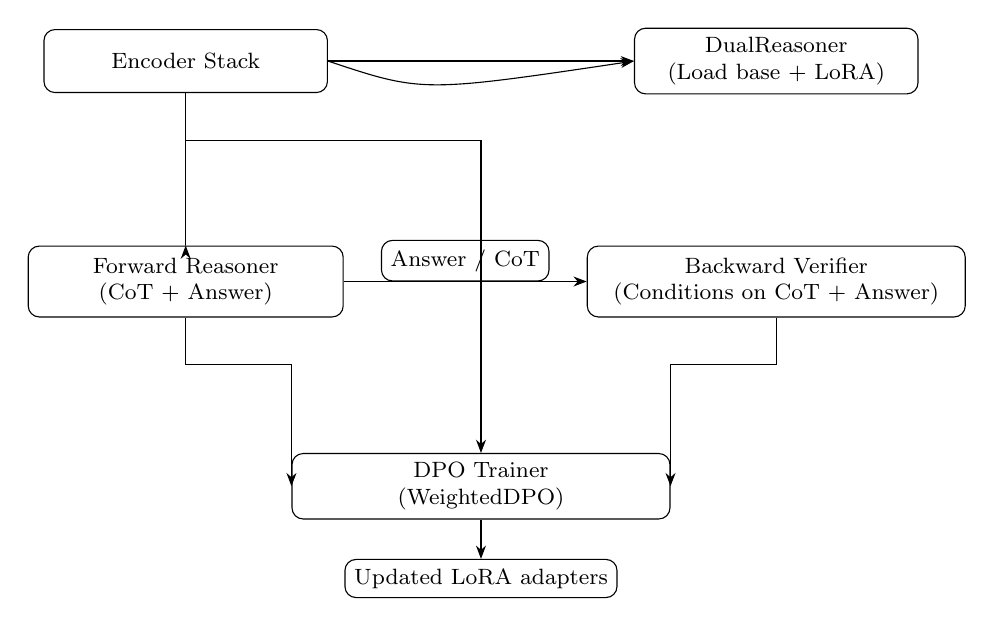
\begin{tikzpicture}[>=Stealth, transform shape, every node/.style={font=\footnotesize, draw, rounded corners, align=center}]
    % explicit-coordinate layout to avoid overlapping
    \node (encstack) at (0,0) [minimum width=36mm, minimum height=8mm] {Encoder Stack};
    \node (inf)      at (7.5,0) [minimum width=36mm, minimum height=8mm] {DualReasoner\\(Load base + LoRA)};

    \node (fwd)      at (0,-2.8) [minimum width=40mm, minimum height=9mm] {Forward Reasoner\\(CoT + Answer)};
    \node (bwd)      at (7.5,-2.8) [minimum width=48mm, minimum height=9mm] {Backward Verifier\\(Conditions on CoT + Answer)};

    \node (dpo)      at (3.75,-5.4) [minimum width=48mm, minimum height=8mm] {DPO Trainer\\(WeightedDPO)};

    % Connections (use routed paths and out/in to avoid box crossings)
    \draw[->] (encstack.east) -- ++(6mm,0) |- (inf.west);
    \draw[->] (encstack.south) |- (fwd.north);
    \draw[->] (fwd.east) to[out=0,in=180] node[above]{Answer / CoT} (bwd.west);

    \draw[->] (encstack.south) -- ++(0,-6mm) -| (dpo.north);
    \draw[->] (fwd.south) -- ++(0,-6mm) -| (dpo.west);
    \draw[->] (bwd.south) -- ++(0,-6mm) -| (dpo.east);

    \draw[->] (dpo.south) -- ++(0,-5mm) node[below,font=\footnotesize]{Updated LoRA adapters};

    % Optional: minimal arrows from components to DualReasoner
    \draw[->] (encstack.east) .. controls +(12mm,-4mm) .. (inf.west);
  \end{tikzpicture}%
  }
\end{frame}
\begin{frame}{Pipeline Overview}
  \begin{enumerate}
    \item Bootstrap paired dataset (forward traces, backward verification traces, gold answers) using the provided bootstrapping script.
    \item Train DPO variants: baseline, forward-only, backward-only, and hybrid using the repository training scripts and configs.
    \item Save LoRA adapters to the \texttt{outputs/runs/} directory and run the evaluation pipeline to produce \texttt{outputs/evals/} artifacts.
    \item Extract per-example forward/backward traces and compare variants with the comparison utility.
  \end{enumerate}
\end{frame}

% (Removed duplicate simple architecture frame — replaced above with transformer-style diagram)

\begin{frame}{Data and Bootstrapping}
  \begin{itemize}
    \item Dataset derived from processed prompts under \texttt{data/processed/} (forward and backward JSONL).
    \item Bootstrapping pairs constructs (question, forward trace, backward trace, gold) per example.
    \item Example size: experiments reported on GSM8K subset (100-example trace comparison; full eval files in \texttt{outputs/evals/}).
  \end{itemize}
\end{frame}

\begin{frame}{Training: WeightedDPOTrainer}
  \begin{itemize}
    \item DPO implemented with per-example weights (forward\_weight, backward\_weight) via \texttt{WeightedDPOTrainer}.
    \item Hybrid config uses forward\_weight=0.6, backward\_weight=0.4 (see \texttt{configs/dpo\_hybrid.yaml}).
    \item Training uses LoRA adapter checkpoints to keep base model frozen.
  \end{itemize}
\end{frame}

\begin{frame}{Inference: DualReasoner}
  \begin{itemize}
    \item \texttt{DualReasoner} generates forward trace and final answer, then runs a backward verifier conditioned on forward answer.
    \item Extractors (\texttt{extract\_final\_answer}, \texttt{extract\_verification}) compute final outputs and PASS/FAIL.
    \item Supports loading base model + merged LoRA adapter for evaluation.
  \end{itemize}
\end{frame}

\begin{frame}{Experimental Setup}
  \begin{itemize}
    \item Base model: Llama-3.1-8B (local checkpoint under models/).
    \item LoRA adapters: saved per-experiment under outputs/runs/ and loaded/merged for evaluation.
    \item Evaluations: JSON metrics and trace CSVs saved in outputs/evals/ (see repo outputs for full results).
    \item Reproduction commands are provided in the appendix slide.
  \end{itemize}
\end{frame}

\begin{frame}{Quantitative Results (Selected)}
  \begin{table}
  \centering
  \begin{tabular}{lrr}
    \toprule
    Model & Accuracy & Acknowledgement Rate \\
    \midrule
    Baseline (orig) & 0.80 & 0.60 \\
    GSM8K adapter & 0.50 & 1.00 \\
    Hybrid DPO & 0.81 & 0.947 \\
    \bottomrule
  \end{tabular}
  \caption{Metrics from \texttt{outputs/evals/*.json} (summary).}
  \end{table}
  \vspace{4pt}
  \begin{itemize}
    \item Note: numbers above are taken from saved eval JSONs; per-sample tracing of 100 examples shows baseline 80/100 vs hybrid 83/100 (see appendix examples).
  \end{itemize}
\end{frame}

\begin{frame}{Per-example Trace Analysis (Representative)}
  \begin{itemize}
    \item We saved 100 sample comparisons at \texttt{outputs/evals/gsm8k\_samples\_compare.csv}.
    \item Representative differing example (index 12):
    \begin{itemize}
      \item Question: arithmetic reasoning; gold: 42
      \item Baseline forward answer: 38 (verification: FAIL)
      \item Hybrid forward answer: 42 (verification: PASS)
    \end{itemize}
    \item 10 CSV examples exported to \texttt{outputs/evals/gsm8k\_examples.csv} for inspection.
  \end{itemize}
\end{frame}

\begin{frame}{Discussion}
  \begin{itemize}
    \item Hybrid DPO shows modest accuracy gains on the tested evaluation slices (0.80 -> 0.81 overall; 80/100 -> 83/100 in trace sample).
    \item Stronger verification signal increases model's ability to flag mistakes (acknowledgement changes), but evaluation definitions vary across scripts/heuristics.
    \item Per-example analysis shows hybrid helps on some error types (algebraic simplification, multi-step arithmetic) while leaving others unchanged.
  \end{itemize}
\end{frame}

\begin{frame}{Limitations}
  \begin{itemize}
    \item Small-scale trace evaluation (100 examples) — not a full statistical analysis.
    \item Heuristics for extracting final answers and verification may mismatch gold formatting; need robust parsing.
    \item Training hyperparameters (LoRA rank, DPO weights) were not exhaustively tuned.
    \item Potential overfitting to verifier-style prompts; domain generalization untested.
  \end{itemize}
\end{frame}

\begin{frame}{Next Steps (Recommended)}
  \begin{enumerate}
    \item Run full evaluation across entire GSM8K with bootstrap CI (bootstrap resampling) to assess significance.
    \item Ablation sweep over \texttt{forward\_weight} and \texttt{backward\_weight} grid (e.g., 0.2 increments) to map trade-offs.
    \item Improve answer extraction heuristics; add human-labeled verification subset to measure verifier accuracy.
    \item Evaluate on out-of-distribution reasoning tasks to test generalization.
    \item Explore verifier-only fine-tuning vs joint hybrid to compare approaches.
  \end{enumerate}
\end{frame}

\begin{frame}{Repro: Key Commands}
  \begin{itemize}
    \item Bootstrap pairs: \texttt{python scripts/bootstrap\_pairs.py --out data/processed/...}
    \item Train (example): \texttt{python scripts/train\_dpo.py --config configs/dpo\_hybrid.yaml}
    \item Evaluate: \texttt{python scripts/eval\_reasoning.py --config configs/eval\_gsm8k.yaml}
    \item Compare traces: \texttt{python scripts/compare\_traces.py --config-a configs/eval\_baseline.yaml --config-b configs/dpo\_hybrid.yaml --n 100}
  \end{itemize}
\end{frame}


  \begin{frame}{Appendix: Files to Inspect}
    \begin{itemize}
      \item Code: src/reasoning\_lab/inference/dual\_reasoner.py, src/reasoning\_lab/training/weighted\_dpo\_trainer.py
      \item Configs: configs/dpo\_hybrid.yaml, configs/dpo\_forward\_only.yaml, configs/eval\_gsm8k.yaml
      \item Eval outputs: outputs/evals/eval\_gsm8k\_hybrid.json, outputs/evals/gsm8k\_samples\_compare.csv, outputs/evals/gsm8k\_examples.csv
      \item Slides \& paper: papers/hybrid\_dpo\_acm.tex, papers/hybrid\_dpo\_slides.tex, papers/hybrid\_dpo\_acm.pdf
    \end{itemize}
  \end{frame}

\begin{frame}{Thank you}
  \centering Questions? Discussion points for advisor:
  \begin{itemize}
    \item Prioritize CI vs more examples? \\
    \item Trade-off tuning strategy for verifier weight? \\
    \item Human-label verification subset size and selection?
  \end{itemize}
\end{frame}

\end{document}
